\lstinline!(make-pair 1 (make-pair!\lstinline! 2 empty))!\\
\uline{Visualisierung Listen}\\ \ \\
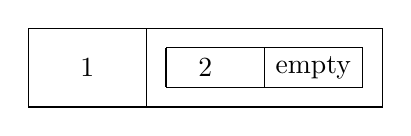
\begin{tikzpicture}
\draw[black,solid] (0,0)--(0,1);
\draw[black,solid] (0,0)--(4.5,0);
\draw[black,solid] (0,1)--(4.5,1);
\draw[black,solid] (4.5,1)--(4.5,0);
\draw[black,solid] (1.5,1)--(1.5,0);
\node () at (0.75,0.5) {1};
\draw[black,solid] (1.75,0.25)--(4.25,0.25);
\draw[black,solid] (1.75,0.75)--(4.25,0.75);
\draw[black,solid] (1.75,0.75)--(1.75,0.25);
\draw[black,solid] (4.25,0.75)--(4.25,0.25);
\node () at (2.25,0.5) {2};
\draw[black,solid] (3.0,0.75)--(3.0,0.25);\\
\node () at (3.62,0.5) {empty};
\end{tikzpicture}\\ \ \\
\includegraphics{katzenbabies}
\uline{Spine (Rückgrat)}\\
\lstinline!(pair-of natural (list-of natural))!\\
\begin{tikzpicture}
\node () at (-1.75,0.5) {\lstinline!(natural first)!};
\node () at (3.5,0.5) {\lstinline! rest (list-of natural)!};
\draw[black,solid] (0,0)--(0,1);
\draw[black,solid] (0,0)--(1,0);
\draw[black,solid] (0,1)--(1,1);
\draw[black,solid] (1,1)--(1,0);
\draw[black,solid] (0.5,1)--(0.5,0);
\node () at (0.25,0.5) {1};
\draw[black,solid] (0.75,0.5)--(1.5,-0.75);
\draw[black,solid] (1.5,-0.75)--(1.5,-1.75);
\draw[black,solid] (1.5,-0.75)--(2.5,-0.75);
\draw[black,solid] (1.5,-1.75)--(2.5,-1.75);
\draw[black,solid] (2.5,-1.75)--(2.5,-0.75);
\draw[black,solid] (2.0,-1.75)--(2.0,-0.75);
\node () at (1.75,-1.25) {2};
\draw[black,solid] (2.25,-1.25)--(3,-2.5);
\node () at (3,-2.75) {\lstinline!empty!};
\end{tikzpicture}\\
\begin{lstlisting}[frame=single]
(: one-to-four (list-of natural))
(define one-two
  (make-pair 1 
             (make-pair 2  
                          empty)))  
\end{lstlisting}
\lstinline!(: jedis-and-siths (list-of (list-of string)))!\bigskip\\ 
\begin{tikzpicture}
\node () at (0,5) {};
\draw (6,6) rectangle (5,5);
\draw[black,solid] (5.5,6)--(5.5,5);
\draw[black,solid] (5.25,5.5)--(4.5,4.5);
\draw[black,solid] (5.75,5.5)--(8.5,4.5);
\draw (8.5,4.5) rectangle (9.5,3.5);
\draw[black,solid] (9.25,4)--(9.8,3.3);
\node () at (9.8,3.1) {\lstinline!empty!};

\draw[black,solid] (8.75,4)--(7.5,3);
\draw (7.5,3) rectangle (8.5,2);
\draw (8,3)--(8,2);
\draw (7.75,2.5)--(7,2);
\node () at (7,1.75) {\textcolor{string}{''Doku''}};

\draw (8.25,2.5)--(9,2);
\draw[black,solid] (9,2) rectangle (10,1);
\draw (9.5,2)--(9.5,1);
\draw (9.75,1.5)--(10.5,0.5);
\node () at (10.5,.25) {\lstinline!empty!};
\draw (9.25,1.5)--(8.75,0.5);
\node () at (8.75,0.25) {\textcolor{string}{''Darth''}};


\draw[black,solid] (9,3.5)--(9,4.5);
\draw (4.5,4.5) rectangle (3.5,3.5);
\draw[black,solid] (4,4.5)--(4,3.5);
\draw (3.75,4)--(3.3,3.3);
\node () at (3.2,3.1) {\textcolor{string}{''Obi''}};
\draw (4.25,4)--(5,2.5);
\draw (5,2.5) rectangle (6,1.5);
\draw (5.5,2.5)--(5.5,1.5);
\draw (5.25,2)--(4.5,1);
\draw (5.75,2)--(6.5,1);
\node () at (4.5,0.8) {\textcolor{string}{''Yoda''}};
\node () at (6.5,0.8) {\lstinline!empty!};
\end{tikzpicture}
\racket{Geschachtelte Listen}{Jedis und Siths in einer geschachtelten Liste}{nestedlist}
\uline{Prozeduren, die Liste konsumieren}\\
Konstruktionsanleitung:\\
Beispiel:\\
\begin{lstlisting}
(: list-sum ((list-of number) -> number))

(check-expect (list-sum empty) 0)
(check-expect (list-sum (make-pair 40
                                   (make-pair 2
                                              empty))) 42)  
(check-expect (list-sum one-to-four) 10)

(define list-sum
  (lambda (xs)
    (cond ((empty? xs) 0)
          ((pair? xs) (+ (first xs)
                         (@{\uline{list-sum} (rest xs)))))))
\end{lstlisting}
\begin{figure}[htbp]
\begin{minipage}[b]{\textwidth}
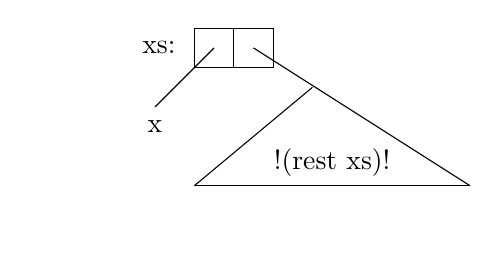
\begin{tikzpicture}
\node () at (0,0) {};
\draw (2,2) rectangle (3,2.5);
\node () at (1.55,2.25) {xs:};
\draw (2.5,2.5)--(2.5,2);
\draw (2.25,2.25)--(1.5,1.5);
\node () at (1.5,1.25) {x};
\draw (2.75,2.25)--(5.5,0.5);
\draw (3.5,1.75)--(2,0.5);
\draw (2,0.5)--(5.5,0.5);
\node () at (3.75,0.8) {\lstinline!(rest xs)!};
\end{tikzpicture}
\hspace*{2cm}
\begin{minipage}[b]{0.3\textwidth}
\lstinline!(rest xs)! mit Signatur \lstinline!(list-of number)! ist selbst wieder eine \uline{kürzere} \uline{Liste} von Zahlen.\\
\lstinline!(list sum (rest xs))! erzielt Fortschritt
\end{minipage}
\end{minipage}
\end{figure}
Konstruktionsanleitung für Prozeduren:
\begin{lstlisting}
(: <f> ((list-of @\argt{1}@) -> @\argt{2}@))
(define <f>
	(lambda(xs)
		(cond 
			((empty? xs) ...)
			((pair? xs) ... @$\overbrace{\text{(first xs)}}^{\text{\argt{1}}}$@ ...)
				(<f> @$\underbrace{\text{(rest xs )}}_{\text{\argt{1}}}$@))...))
\end{lstlisting}
Neue Sprachebene ''Macht der Abstraktion''
\begin{enumerate}[-]
\i Signatur \lstinline!(list-of \% a)! eingebaut
\begin{lstlisting}
(list @\arge{1}@ @\arge{2}@ ... @\arge{n}@)
	@$\equiv$@
(make-pair (@\arge{1}@)
	(make-pair @\arge{2}@)
		... (make-pair @\arge{n}@) empty) ...)
\end{lstlisting}
\i Ausgabeformat für nicht leere Listen:\\
\lstinline!{#<list x1 x2 ... xn>!
\end{enumerate}
\racket{Rekursion auf Listen: Länge einer Liste}{Länge einer Liste}{recursivelistlength}
Füge Listen xs , ys zusammen (con\uline{cat}ination)\\
Zwei Fälle (xs leer oder nicht leer)
\begin{enumerate}
\i[\circled{1}] $\overbrace{ \text{\lstinline!empty!}}^{\text{xs}} \ \ \overbrace{y_1 \ y_2 \ \ldots \ y_m}^{ys}
 \ \ \overbrace{y_1 \ y_2 \ \ldots \ y_m}^{\text{\lstinline!(cat \ xs \ ys)!}}$
\i[\circled{2}] $x_1 \ \underbrace{x_2 \ \ldots \ x_n}_{\text{\lstinline!(rest xs)!}} \ y_1 \ y_2 \ \ldots \ y_m \ \ x_1 \ \underbrace{ x_2 \ldots \ x_n \ y_1 \ y_2 \ \ldots \ y_m}_{\text{\lstinline!(cat rest xs)!}}$
\end{enumerate}

Beobachtung:
\begin{enumerate}[-]
\i Die Längen von xs bestimmt die Anzahl der rekursiven Aufrufe von cat
\i Auf xs werden \uline{Selektoren angewendet}
\end{enumerate}
\racket{Rekursion: Zusammenfügen zweier Listen}{Zusammenfügen zweier Listen}{cat}
\pagebreak